%*******************************************************
% Abstract+Sommario
%*******************************************************

\pdfbookmark{Abstract}{Abstract}
\begingroup
\let\clearpage\relax
\let\cleardoublepage\relax
\let\cleardoublepage\relax

\chapter*{Synopsis}
Dorel Industries was established in 1962, and consists of 3 major divisions (Juvenile, Home Furnishings, and Recreational/Leisure) \cite{DorelIndustries2013}.  It owns a wide array of strong brands, including Cosco, Schwinn, Ironhorse, and Mongoose.  While Dorel is a strong player in the bicycle industry, it recently announced (In January of this year) that it would be shuttering its bicycle assembly facilities in the United States and moving to Asia in order to become more competitive \cite{Marotte2014}.  Annual sales are roughly \$2.6 billion, and with a restructuring of the Recreational/Leisure unit, Dorel expects to save at least \$6 million annually \cite{Carpiet2014}.  Dorel’s primary competitors include Kid Brands, Inc., Trek Bicycle Corporation, and Evenflo Company, Inc \cite{Hoovers2014}.  Dorel currently employs 6,300 people in facilities located in twenty-four countries worldwide.

\vfill
{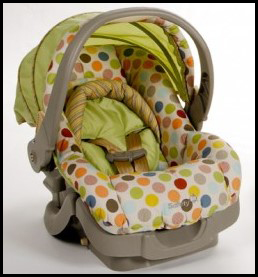
\includegraphics[width=.45\columnwidth]{baby}} 
{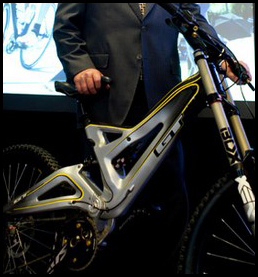
\includegraphics[width=.45\columnwidth]{bike}} 
\vfill
\selectlanguage{american}
\pdfbookmark[1]{StrategicIssues}{StrategicIssues}
\chapter*{Strategic Issues}

\begin{itemize}
  \item Competitors have already outsourced to Asia \cite{VoiceofAmerica2009}.
  \item Fourth quarter earnings are much lower than levels last year due to reduced bicycle sales.  Dorel reported that its retailers received fewer customers over the holidays than average \cite{Symon2014}.
  \item Currently have an unrelated portfolio amongst business units.
  \item Cash cow (Home Furnishings) is losing revenue YOY.
  \item Unfavorable foreign exchange rates reducing net profits \cite{Symon2014}.
  \item The board believes the company’s market price is currently undervalued.
  \item One more Item.
\end{itemize}

\pdfbookmark[2]{Options}{Options}
\chapter*{Options}


\begin{enumerate}
  \item Focus on outsourcing and cutting costs, compete on price.
  \item Continue global expansion, specifically on elevating the recreational / bicycle unit by acquiring popular brands in each region.
  \item Refocus on premium products, drop cheap brands (Pacific Cycle etc.) that conflict with company identity and differentiate on quality.
\end{enumerate}





\selectlanguage{american}

\endgroup			

\vfill

